\documentclass[11pt,preprint]{elsarticle}

\usepackage{lmodern}
%%%% My spacing
\usepackage{setspace}
\setstretch{1.2}
\DeclareMathSizes{12}{14}{10}{10}

% Wrap around which gives all figures included the [H] command, or places it "here". This can be tedious to code in Rmarkdown.
\usepackage{float}
\let\origfigure\figure
\let\endorigfigure\endfigure
\renewenvironment{figure}[1][2] {
    \expandafter\origfigure\expandafter[H]
} {
    \endorigfigure
}

\let\origtable\table
\let\endorigtable\endtable
\renewenvironment{table}[1][2] {
    \expandafter\origtable\expandafter[H]
} {
    \endorigtable
}


\usepackage{ifxetex,ifluatex}
\usepackage{fixltx2e} % provides \textsubscript
\ifnum 0\ifxetex 1\fi\ifluatex 1\fi=0 % if pdftex
  \usepackage[T1]{fontenc}
  \usepackage[utf8]{inputenc}
\else % if luatex or xelatex
  \ifxetex
    \usepackage{mathspec}
    \usepackage{xltxtra,xunicode}
  \else
    \usepackage{fontspec}
  \fi
  \defaultfontfeatures{Mapping=tex-text,Scale=MatchLowercase}
  \newcommand{\euro}{€}
\fi

\usepackage{amssymb, amsmath, amsthm, amsfonts}

\def\bibsection{\section*{References}} %%% Make "References" appear before bibliography


\usepackage[numbers]{natbib}

\usepackage{longtable}
\usepackage[margin=2.3cm,bottom=2cm,top=2.5cm, includefoot]{geometry}
\usepackage{fancyhdr}
\usepackage[bottom, hang, flushmargin]{footmisc}
\usepackage{graphicx}
\numberwithin{equation}{section}
\numberwithin{figure}{section}
\numberwithin{table}{section}
\setlength{\parindent}{0cm}
\setlength{\parskip}{1.3ex plus 0.5ex minus 0.3ex}
\usepackage{textcomp}
\renewcommand{\headrulewidth}{0.2pt}
\renewcommand{\footrulewidth}{0.3pt}

\usepackage{array}
\newcolumntype{x}[1]{>{\centering\arraybackslash\hspace{0pt}}p{#1}}

%%%%  Remove the "preprint submitted to" part. Don't worry about this either, it just looks better without it:
\makeatletter
\def\ps@pprintTitle{%
  \let\@oddhead\@empty
  \let\@evenhead\@empty
  \let\@oddfoot\@empty
  \let\@evenfoot\@oddfoot
}
\makeatother

 \def\tightlist{} % This allows for subbullets!

\usepackage{hyperref}
\hypersetup{breaklinks=true,
            bookmarks=true,
            colorlinks=true,
            citecolor=blue,
            urlcolor=blue,
            linkcolor=blue,
            pdfborder={0 0 0}}


% The following packages allow huxtable to work:
\usepackage{siunitx}
\usepackage{multirow}
\usepackage{hhline}
\usepackage{calc}
\usepackage{tabularx}
\usepackage{booktabs}
\usepackage{caption}


\newenvironment{columns}[1][]{}{}

\newenvironment{column}[1]{\begin{minipage}{#1}\ignorespaces}{%
\end{minipage}
\ifhmode\unskip\fi
\aftergroup\useignorespacesandallpars}

\def\useignorespacesandallpars#1\ignorespaces\fi{%
#1\fi\ignorespacesandallpars}

\makeatletter
\def\ignorespacesandallpars{%
  \@ifnextchar\par
    {\expandafter\ignorespacesandallpars\@gobble}%
    {}%
}
\makeatother


% definitions for citeproc citations
\NewDocumentCommand\citeproctext{}{}
\NewDocumentCommand\citeproc{mm}{%
\href{\#cite.\detokenize{#1}}{#2}\nocite{#1}}

\makeatletter
% allow citations to break across lines
\let\@cite@ofmt\@firstofone
% avoid brackets around text for \cite:
\def\@biblabel#1{}
\def\@cite#1#2{{#1\if@tempswa , #2\fi}}
\makeatother
\newlength{\cslhangindent}
\setlength{\cslhangindent}{1.5em}
\newlength{\csllabelwidth}
\setlength{\csllabelwidth}{3em}
\newenvironment{CSLReferences}[2] % #1 hanging-indent, #2 entry-spacing
{\begin{list}{}{%
	\setlength{\itemindent}{0pt}
	\setlength{\leftmargin}{0pt}
	\setlength{\parsep}{0pt}
	% turn on hanging indent if param 1 is 1
	\ifodd #1
	\setlength{\leftmargin}{\cslhangindent}
	\setlength{\itemindent}{-1\cslhangindent}
	\fi
	% set entry spacing
	\setlength{\itemsep}{#2\baselineskip}}}
{\end{list}}

\usepackage{calc}
\newcommand{\CSLBlock}[1]{\hfill\break\parbox[t]{\linewidth}{\strut\ignorespaces#1\strut}}
\newcommand{\CSLLeftMargin}[1]{\parbox[t]{\csllabelwidth}{\strut#1\strut}}
\newcommand{\CSLRightInline}[1]{\parbox[t]{\linewidth - \csllabelwidth}{\strut#1\strut}}
\newcommand{\CSLIndent}[1]{\hspace{\cslhangindent}#1}


\urlstyle{same}  % don't use monospace font for urls
\setlength{\parindent}{0pt}
\setlength{\parskip}{6pt plus 2pt minus 1pt}
\setlength{\emergencystretch}{3em}  % prevent overfull lines
\setcounter{secnumdepth}{5}

%%% Use protect on footnotes to avoid problems with footnotes in titles
\let\rmarkdownfootnote\footnote%
\def\footnote{\protect\rmarkdownfootnote}
\IfFileExists{upquote.sty}{\usepackage{upquote}}{}

%%% Include extra packages specified by user

%%% Hard setting column skips for reports - this ensures greater consistency and control over the length settings in the document.
%% page layout
%% paragraphs
\setlength{\baselineskip}{12pt plus 0pt minus 0pt}
\setlength{\parskip}{12pt plus 0pt minus 0pt}
\setlength{\parindent}{0pt plus 0pt minus 0pt}
%% floats
\setlength{\floatsep}{12pt plus 0 pt minus 0pt}
\setlength{\textfloatsep}{20pt plus 0pt minus 0pt}
\setlength{\intextsep}{14pt plus 0pt minus 0pt}
\setlength{\dbltextfloatsep}{20pt plus 0pt minus 0pt}
\setlength{\dblfloatsep}{14pt plus 0pt minus 0pt}
%% maths
\setlength{\abovedisplayskip}{12pt plus 0pt minus 0pt}
\setlength{\belowdisplayskip}{12pt plus 0pt minus 0pt}
%% lists
\setlength{\topsep}{10pt plus 0pt minus 0pt}
\setlength{\partopsep}{3pt plus 0pt minus 0pt}
\setlength{\itemsep}{5pt plus 0pt minus 0pt}
\setlength{\labelsep}{8mm plus 0mm minus 0mm}
\setlength{\parsep}{\the\parskip}
\setlength{\listparindent}{\the\parindent}
%% verbatim
\setlength{\fboxsep}{5pt plus 0pt minus 0pt}



\begin{document}



\begin{frontmatter}  %

\title{22894551 - Question 1 - I was named after WHO?}

% Set to FALSE if wanting to remove title (for submission)




\author[Add1]{Charisa Geyer}
\ead{22894551@sun.ac.za}





\address[Add1]{Stellenbosch University, Cape Town, South Africa}


\begin{abstract}
\small{
This report shows trends in US baby names. It looks at persistence and
populatarity of baby names and its correlation to other popular US
celebrities and Netflix/ TV shows over the decades.
}
\end{abstract}

\vspace{1cm}





\vspace{0.5cm}

\end{frontmatter}

\setcounter{footnote}{0}



%________________________
% Header and Footers
%%%%%%%%%%%%%%%%%%%%%%%%%%%%%%%%%
\pagestyle{fancy}
\chead{}
\rhead{}
\lfoot{}
\rfoot{\footnotesize Page \thepage}
\lhead{}
%\rfoot{\footnotesize Page \thepage } % "e.g. Page 2"
\cfoot{}

%\setlength\headheight{30pt}
%%%%%%%%%%%%%%%%%%%%%%%%%%%%%%%%%
%________________________

\headsep 35pt % So that header does not go over title




\section{\texorpdfstring{Introduction
\label{Introduction}}{Introduction }}\label{introduction}

The Toy Store wants to know if there are trends in naming conventions.
Parents get influenced by the media, tradition and other unknown
factors. If trends are persistent, the Toy Store can rely on trends to
cater their toy names to. \newpage

\section{Plot 1: Most popular names over the
years}\label{plot-1-most-popular-names-over-the-years}

We observe the popularity of names for boys and girls over time. By
looking at the colour-coordinated bubbles, we observe persistence in the
naming of very popular names like ``Mary'' and ``James'' - the two most
popular names overall.

\begin{center}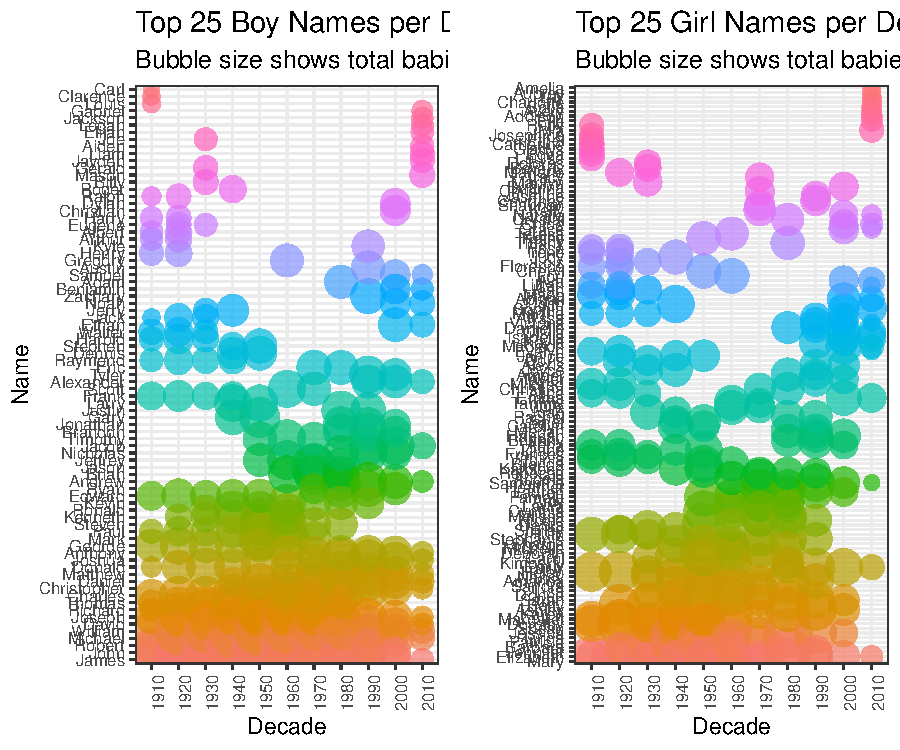
\includegraphics{Question1_files/figure-latex/unnamed-chunk-1-1} \end{center}
\newpage

\section{Plot 2: Increase in name popularity year-on-year, per decade
for
Girls}\label{plot-2-increase-in-name-popularity-year-on-year-per-decade-for-girls}

These plots show how year-on-year popularity of names are distributed.
The 3 names that had the highest uptake per decade is shown in red. This
can be compared to releases of music. movies where the name is used. In
early days, parents really did not look further than the first page of
the ``Baby Name Book''.
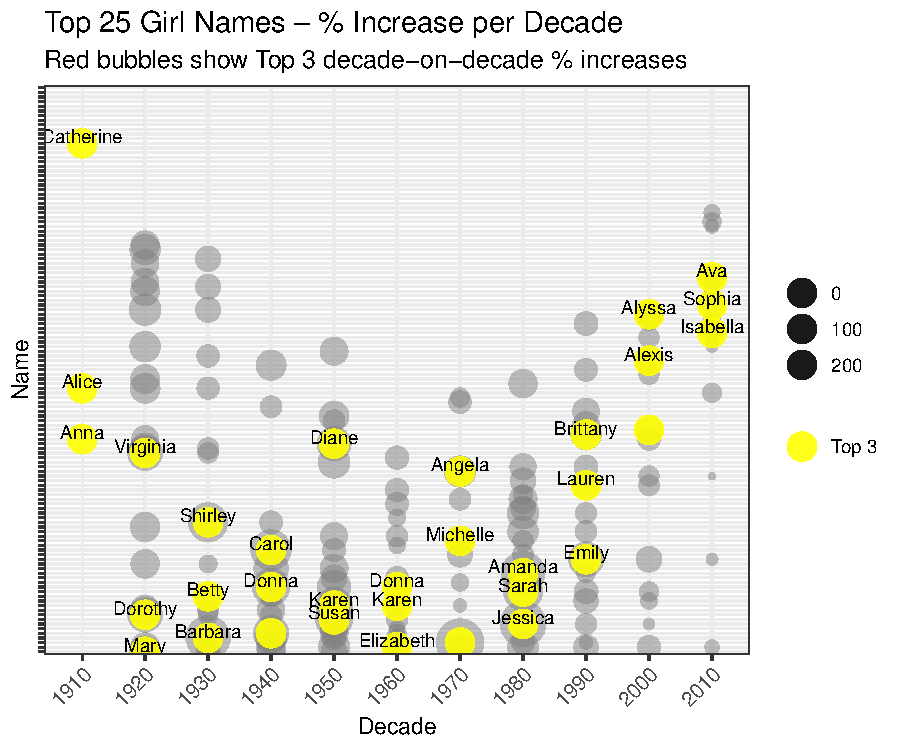
\includegraphics{Question1_files/figure-latex/unnamed-chunk-2-1.pdf}
\newpage

\section{Plot 3: Increase in name popularity year-on-year, per decade
for
boys}\label{plot-3-increase-in-name-popularity-year-on-year-per-decade-for-boys}

These plots show how year-on-year popularity of names are distributed.
The 3 names that had the highest uptake per decade is shown in red. This
can be compared to releases of music. movies where the name is used.
Parents still looked at A-names, and keep on naming their boys names
from the Bible. What is not seen here is the persistence of the name
``James'' Since it remains popular year-on-year, the increase may be
less pertinent.
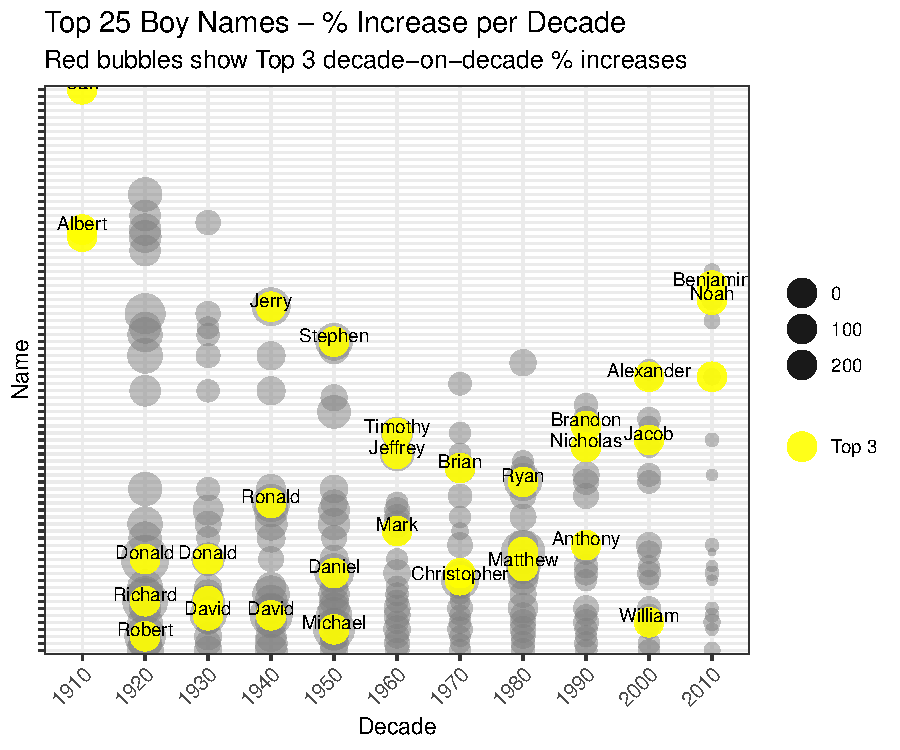
\includegraphics{Question1_files/figure-latex/unnamed-chunk-3-1.pdf}

\newpage

\section{Plot 4: Spearman
correlation}\label{plot-4-spearman-correlation}

\begin{figure}
\centering
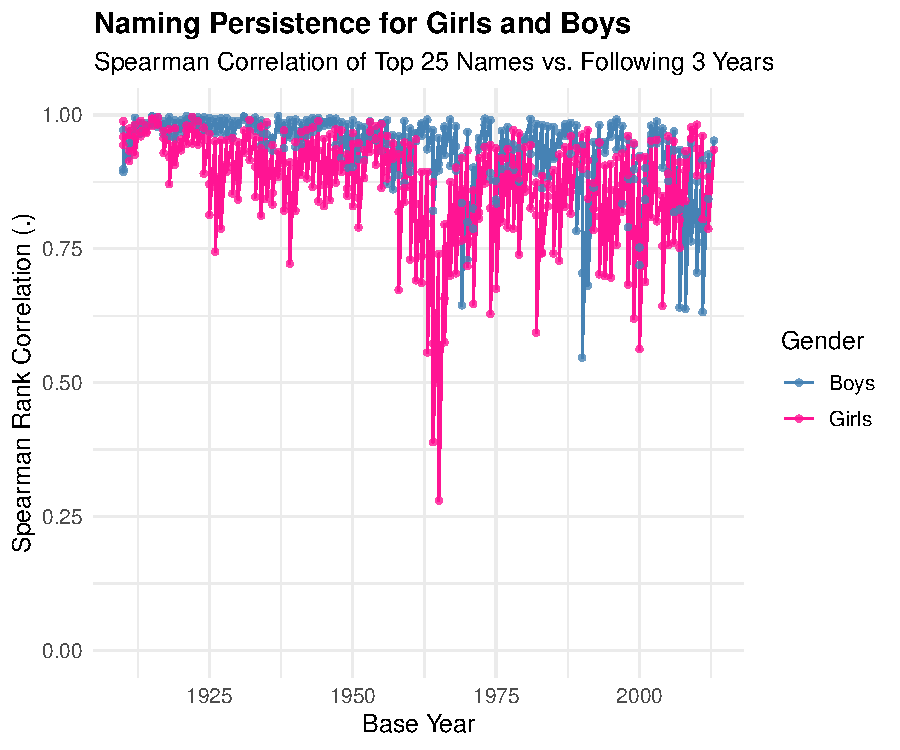
\includegraphics{Question1_files/figure-latex/fig.spearman-1.pdf}
\caption{Figure: Spearman correlation for naming persistence over time}
\end{figure}

We can observe the Spearman rank correlations, portraying naming
persistence of the Top 25girls and boys names in Figure
@ref(fig:spearman). In the early years, naming persistence was very
high, with a correlation close to 1. Naming persistence decreased
severely in the 1960s and stayed lower. For girls, it also decreased,
but not as dramatically. Between the 1970s and 1990s, naming patterns in
the United States began to shift noticeably, particularly for girls. The
rise of television, pop music, and mass media exposed parents to a wider
range of influences. Parents were now getting inspiration from soap
opera characters to chart-topping musicians --- which led to short-lived
spikes in name popularity
(\citeproc{ref-abramson2003TVhistory}{Abramson, 2003}). Names like
Katina (influenced by the 1974 soap ``Where the Heart Is'') illustrate
how easily cultural moments could shape naming choices. This era marked
a move away from traditional, family-based naming toward more
trend-driven and individualistic preferences, contributing to a clear
decline in naming persistence as measured by year-over-year Spearman
correlations. This leads us to looking into the correlation between the
Top-100 Billoard artist names and HBO character and actor names, with
popular baby names in the US.

\newpage

\section{Comparison with Musicians, Song Titles and Prominent
Figures}\label{comparison-with-musicians-song-titles-and-prominent-figures}

Popular names such as Dorothy and Elizabeth are likely to be based on
political figures, Queen Elizabeth and Dorothy is strongly associated
with the character Dorothy Gale from ``The Wizard of Oz,'' further
solidifying its place in popular culture. The 1939 film adaptation
starring Judy Garland cemented the name's popularity. Barbara Stanwyck
was establishing herself as a prominent film actress, appearing in
popular movies like ``Stella Dallas''.

The most popular boys' names remain those of the 12 disciples in the
Bible.

I would advise the Toy Store to reconsider relying on celebrity names as
a predictor of baby names, but rather rely on most common names to date.

\begin{table}[H]
\centering
\caption{Names in Music, Film and Culture \label{tab:names}} 
\begin{tabular}{lll}
  \hline
Name & Type & Example \\ 
  \hline
Donna & Song name & "Donna" - Ritchie Valens \\ 
  Dorothy & Character & Dorothy Gale - The Wizard of Oz \\ 
  Diane & Song & "Jack and Diane" - John Mellencamp \\ 
  Barbara & Actress & Barbra Streisand \\ 
  Elizabeth & Public figure & Queen Elizabeth \\ 
   \hline
\end{tabular}
\end{table}

\section*{References}\label{references}
\addcontentsline{toc}{section}{References}

\phantomsection\label{refs}
\begin{CSLReferences}{1}{1}
\bibitem[\citeproctext]{ref-abramson2003TVhistory}
Abramson, A. 2003. \emph{The history of television, 1942 to 2000}.
McFarland.

\end{CSLReferences}

\bibliography{Tex/ref}





\end{document}
